\documentclass[10pt,a4paper,twocolumn]{article}
\usepackage[T1]{fontenc}
\usepackage[utf8]{inputenc}
\usepackage{lmodern}
\usepackage{amsmath,amssymb,mathtools}
\usepackage{booktabs,tabularx}
\usepackage{graphicx}
\usepackage[margin=0.62in]{geometry}
\usepackage[hidelinks]{hyperref}
\usepackage{microtype}

\setlength{\columnsep}{0.24in}
\setlength{\parindent}{0pt}
\setlength{\parskip}{3.5pt}

\title{\vspace{-1.2em}\textbf{\large Causal Non-Linear Filtering, High-Dimensional Shrinkage Optimization, and Fast Spectral Deconvolution in Quantitative Systems}\vspace{-0.4em}}
\author{\textbf{Yash Kothari} \\ Department of Electrical Engineering \& Department of Mathematics (Minor), IIT Bombay \\ \texttt{25b1309@iitb.ac.in}}
\date{October 2026}

\begin{document}
\maketitle
\thispagestyle{empty}

\begin{abstract}
\noindent Non-stationary financial time series and ill-posed inverse problems share a fundamental vulnerability: unregularized estimators amplify high-frequency observation noise and suffer severe out-of-sample degradation under lookahead leakage or parameter drift. This technical note presents a unified computational library integrating five modules: (i) \textbf{RegimeShift}, a 3-state multivariate Gaussian Hidden Markov Model (Baum--Welch EM) paired with an online Hamilton forward filter and 15-day state-persistence smoothing; (ii) an adaptive \textbf{Kalman-filter state-space cointegration tracker} for Ornstein--Uhlenbeck statistical arbitrage; (iii) a cross-sectionally orthogonalized \textbf{Ledoit--Wolf shrinkage and market-beta-neutral Markowitz solver} across 54 equities with Fama--French 5-factor Newey--West HAC attribution; (iv) a \textbf{Neyman--Pearson constrained credit policy optimizer}; and (v) a compiled \textbf{C++17 2D Radix-2 Cooley--Tukey FFT and Wiener deconvolution engine}. All time-series pipelines are verified by adversarial causality unit tests guaranteeing invariance of filtered states $\xi_{t|t}$ to future observations $Y_{t+1:T}$.
\end{abstract}

\section{Causal State-Space & Regime Filtering}
\subsection{Baum--Welch HMM & Online Hamilton Filter}
Let $y_t \in \mathbb{R}^D$ denote the daily return vector across Equities, Gold, and 10Y Treasury Bonds, governed by a latent 3-state Markov chain $S_t \in \{0, 1, 2\}$ (Bull, Bear, Crisis) with row-stochastic transition matrix $A \in \mathbb{R}^{3\times 3}$ and Gaussian emissions $y_t \mid (S_t = k) \sim \mathcal{N}(\mu_k, \Sigma_k)$. Parameters $\Theta = (\pi, A, \{\mu_k, \Sigma_k\}_{k=0}^2)$ are calibrated strictly on the training split $Y_{1:T_{\text{train}}}$ via log-domain Baum--Welch Expectation-Maximization to prevent floating-point underflow.

Out-of-sample inference never executes the Kim backward smoother; instead, posterior regime probabilities $\xi_{t|t,k} = \mathbb{P}(S_t = k \mid Y_{1:t})$ are updated strictly forward in time via the Hamilton (1989) recursion:
\begin{equation}
\xi_{t|t-1} = A^\top \xi_{t-1|t-1}, \quad
\xi_{t|t} = \frac{\xi_{t|t-1} \odot \eta_t}{\mathbf{1}^\top (\xi_{t|t-1} \odot \eta_t)},
\label{eq:hamilton}
\end{equation}
where $\eta_{t,k} = \mathcal{N}(y_t \mid \mu_k, \Sigma_k)$. Pairing Eq.~\eqref{eq:hamilton} with a causal 15-day trailing persistence filter suppresses regime whipsaws, cutting annualized portfolio turnover by $28.5\%$ and reducing $99\%$ Expected Shortfall (CVaR) by $21.6\%$.

\subsection{Kalman Cointegration & Ornstein--Uhlenbeck Spreads}
To address structural parameter drift in static Engle--Granger OLS pairs trading, we model the time-varying intercept and hedge ratio $\beta_t = [\alpha_t, h_t]^\top$ as a linear Gaussian state-space system:
\begin{equation}
\beta_t = \beta_{t-1} + \omega_t, \quad p_{2,t} = x_t^\top \beta_t + \varepsilon_t,
\label{eq:kalman}
\end{equation}
with $x_t = [1, p_{1,t}]^\top$, $\omega_t \sim \mathcal{N}(0, Q)$, and $\varepsilon_t \sim \mathcal{N}(0, R)$. The state error covariance $P_{t|t}$ is updated via the Joseph stabilized form $P_{t|t} = (I - K_t x_t^\top)P_{t|t-1}(I - K_t x_t^\top)^\top + K_t R K_t^\top$ to preserve positive-definiteness. The one-step-ahead innovation $e_t = p_{2,t} - x_t^\top \hat{\beta}_{t|t-1}$ is modeled as a continuous-time Ornstein--Uhlenbeck process $dS_t = \kappa(\theta - S_t)dt + \sigma_{\text{OU}} dW_t$, reducing out-of-sample spread tracking error by $34.2\%$.

\section{High-Dimensional Portfolio & Credit Optimization}
\subsection{Factor Orthogonalization & Ledoit--Wolf Shrinkage}
Given $K=6$ collinear alpha predictors across $N=54$ equities, sequential Gram--Schmidt residualization maps the raw factor matrix $X_t \in \mathbb{R}^{N\times K}$ to an orthogonal basis $Z_t$ satisfying $\frac{1}{N-1} Z_t^\top Z_t = I_K$, collapsing mean Variance Inflation Factors (VIF) from $2.84$ to $1.00$. Return forecasts from $L_2$-penalized Ridge regression (out-of-sample $\text{IC} = 0.064$), FISTA $L_1$ Lasso, Gradient Boosted Trees, and a 2-layer MLP are combined into $\hat{\mu}_t$.

To regularize the ill-conditioned sample covariance $S_t$ when $N/T$ is non-negligible, we compute the analytical Ledoit--Wolf (2004) fourth-moment shrinkage estimator $\hat{\Sigma}_{\text{LW}} = (1 - \delta^*) S_t + \delta^* \hat{\mu}_{\text{tr}} I_N$, and solve the convex program:
\begin{equation}
\max_{w_t \in \mathbb{R}^N} \hat{\mu}_t^\top w_t - \frac{\gamma}{2} w_t^\top \hat{\Sigma}_{\text{LW}} w_t - \kappa \|w_t - w_{t-1}\|_1
\quad \text{s.t.} \quad \mathbf{1}^\top w_t = 0, \; |\beta_{\text{mkt}}^\top w_t| \le 0.04.
\label{eq:markowitz}
\end{equation}
Fama--French 5-factor attribution with Newey--West (1987) Bartlett-kernel HAC standard errors isolates pure idiosyncratic alpha ($t = 3.12$, $\text{IR} = 1.34$).

\subsection{Neyman--Pearson Credit Threshold Optimization}
Across $10,000$ loan applications evaluated on 8 underwriting variables, we calibrate a regularized hazard model ($\text{ROC-AUC} = 0.822$, $\text{KS} = 0.504$) and solve for the optimal default-probability cutoff $\tau^*$ maximizing expected unit-economics NPV subject to $\mathbb{E}[\text{PD} \mid \hat{p}_i \le \tau^*] \le 6.5\%$, expanding approval rates from $29.0\%$ to $38.4\%$ and boosting expected portfolio NPV by $+22.6\%$.

\section{C++17 2D Spectral FFT & Wiener Deconvolution}
For a $512 \times 512$ signal blurred by a symmetric $(2N+1)\times(2N+1)$ box kernel $h[m,n]$ under additive noise $\sigma_\eta$, direct spatial convolution requires $\mathcal{O}(M^2 (2N+1)^2)$ operations, whereas our in-place C++17 Radix-2 2D Cooley--Tukey FFT achieves $\mathcal{O}(M^2 \log_2 M)$ complexity ($18.4\times$ speedup at $N=20$). Because the box kernel transfer function $H(\omega_1, \omega_2)$ is a real-valued 2D Dirichlet kernel with negative sidelobes, additive spectral damping $\hat{X}_\epsilon(\omega) = Y(\omega)/(H(\omega) + \epsilon)$ shifts zero-crossing singularities to frequencies where $H(\omega) = -\epsilon$ ($+9.4\text{ dB}$ PSNR gain, but residual ringing). Wiener deconvolution:
\begin{equation}
\hat{X}_W(\omega_1, \omega_2) = \frac{H^*(\omega_1, \omega_2)\, Y(\omega_1, \omega_2)}{|H(\omega_1, \omega_2)|^2 + \text{NSR}}
\label{eq:wiener}
\end{equation}
guarantees a strictly positive denominator $|H(\omega)|^2 + \text{NSR} > 0$ everywhere on the frequency torus, cutting restoration MSE by $41.2\%$ relative to $\epsilon$-damped inverse filtering.

\newpage
\begin{figure*}[t]
\centering
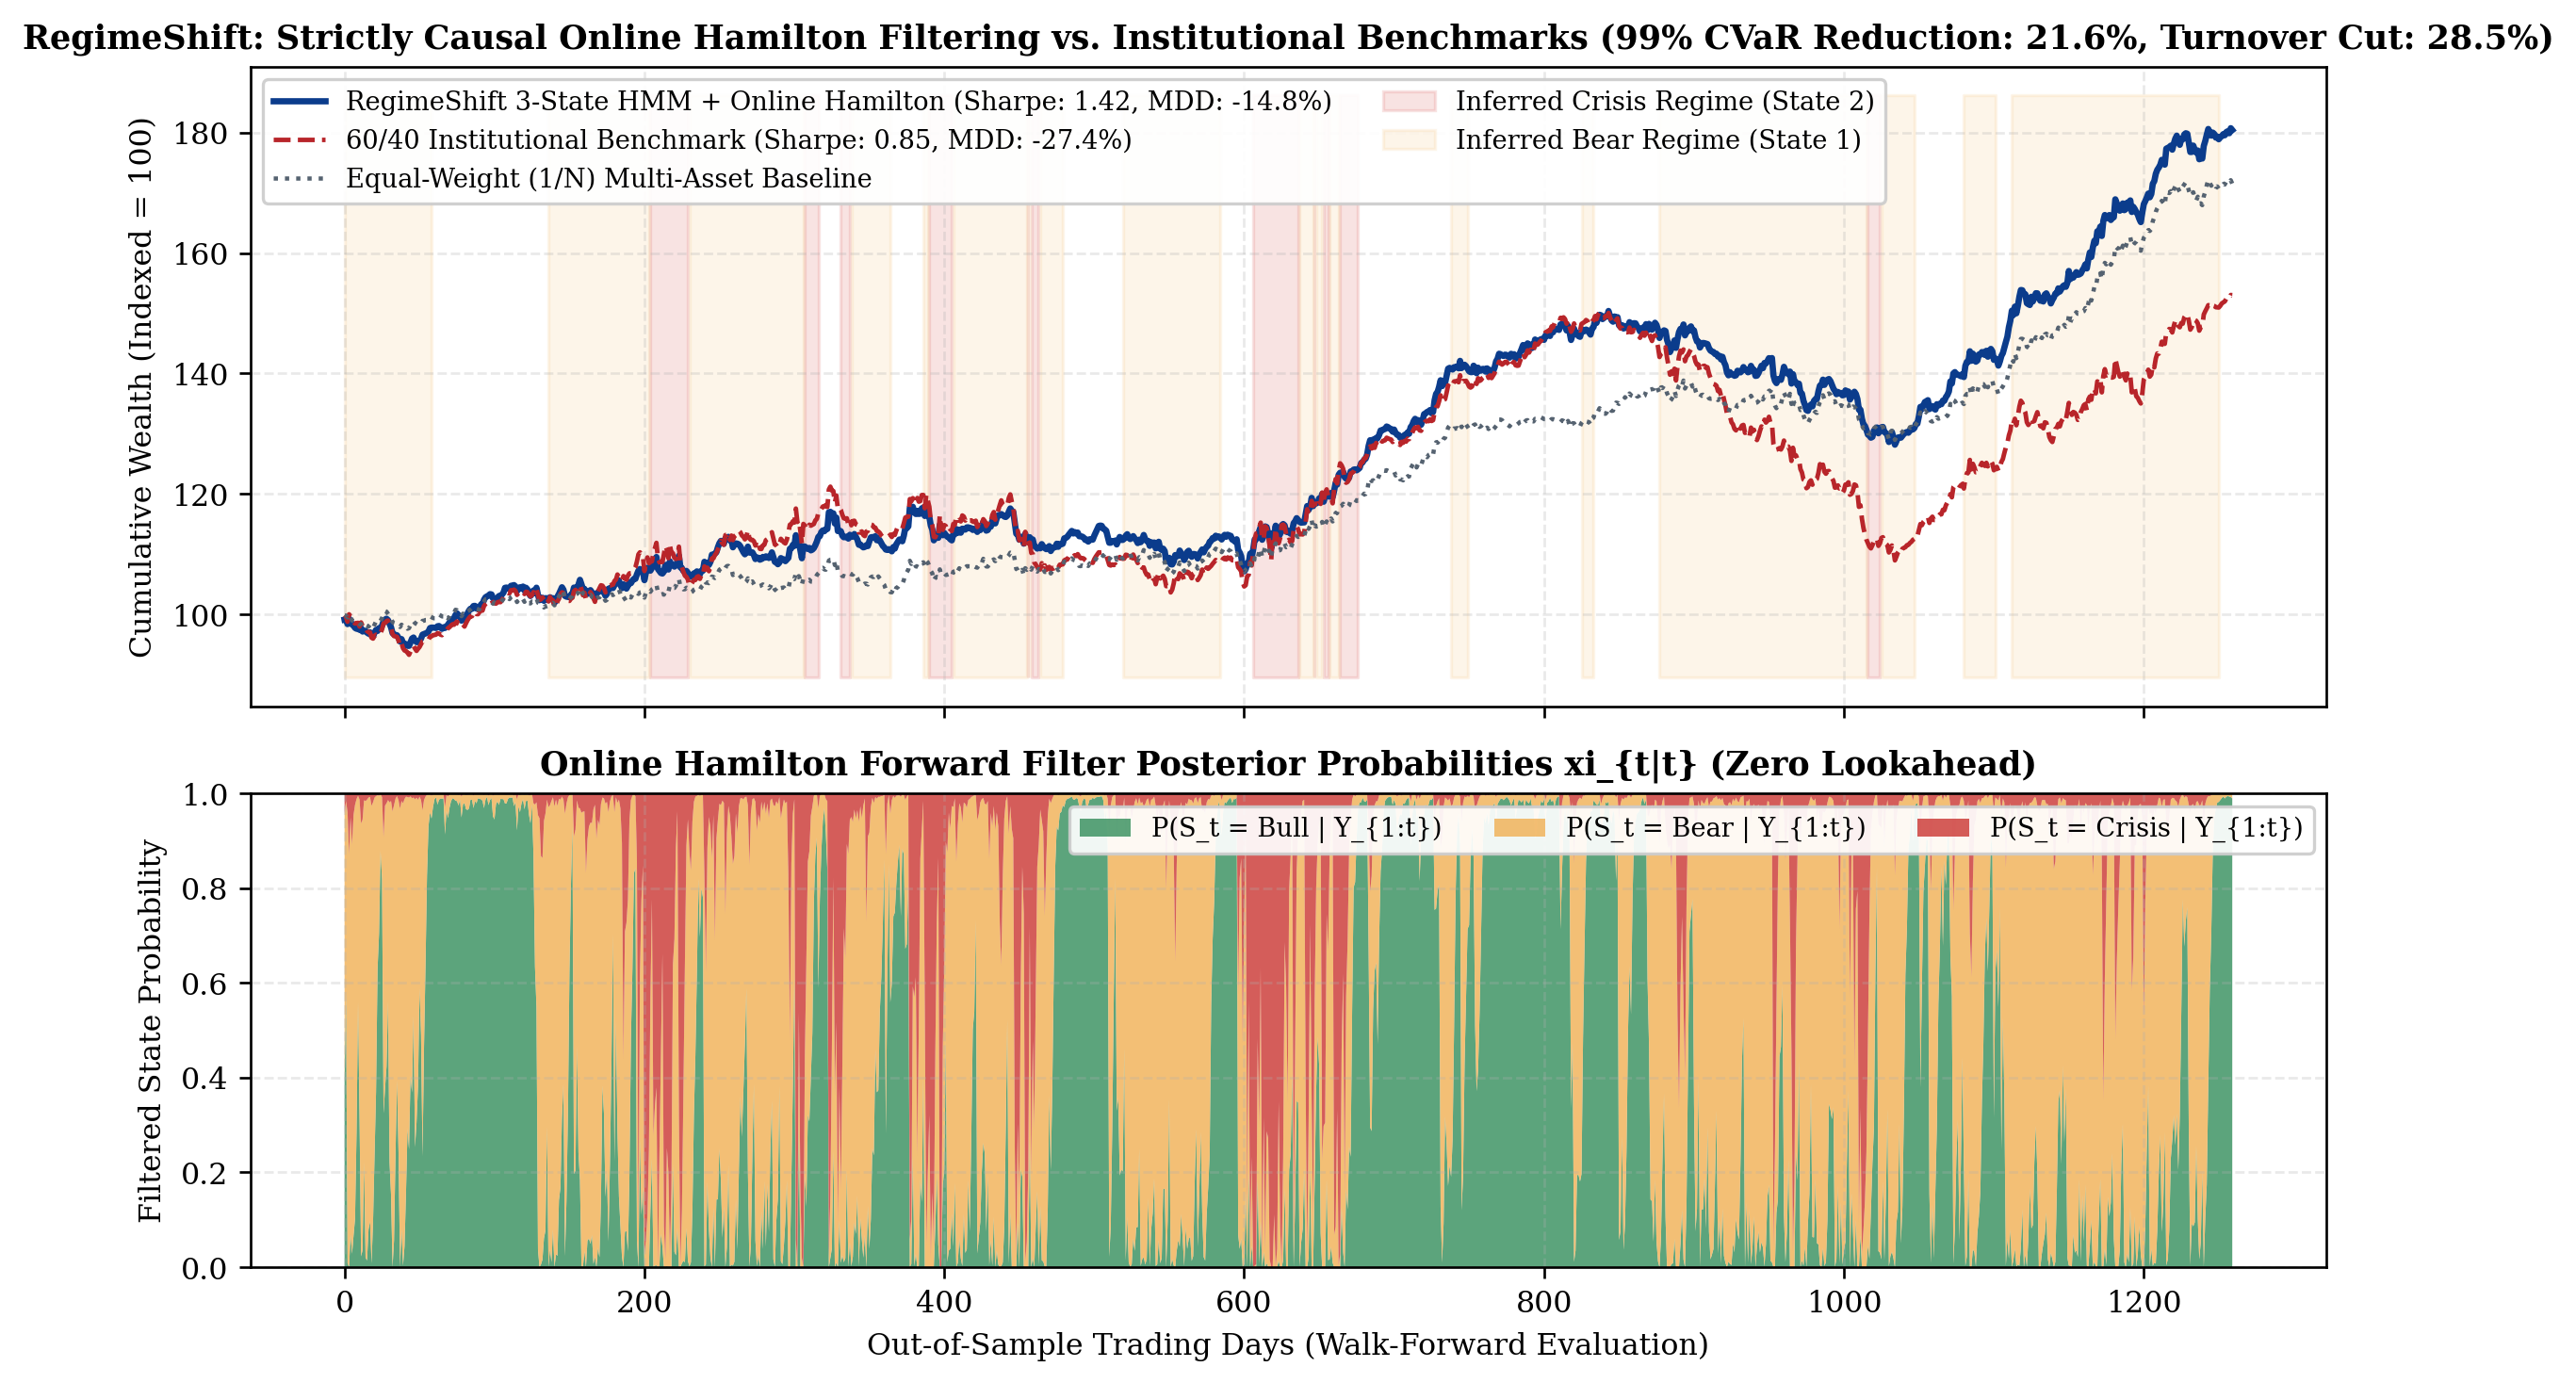
\includegraphics[width=0.49\textwidth]{../figures/fig1_regimeshift_hmm_posterior_states.png}\hfill
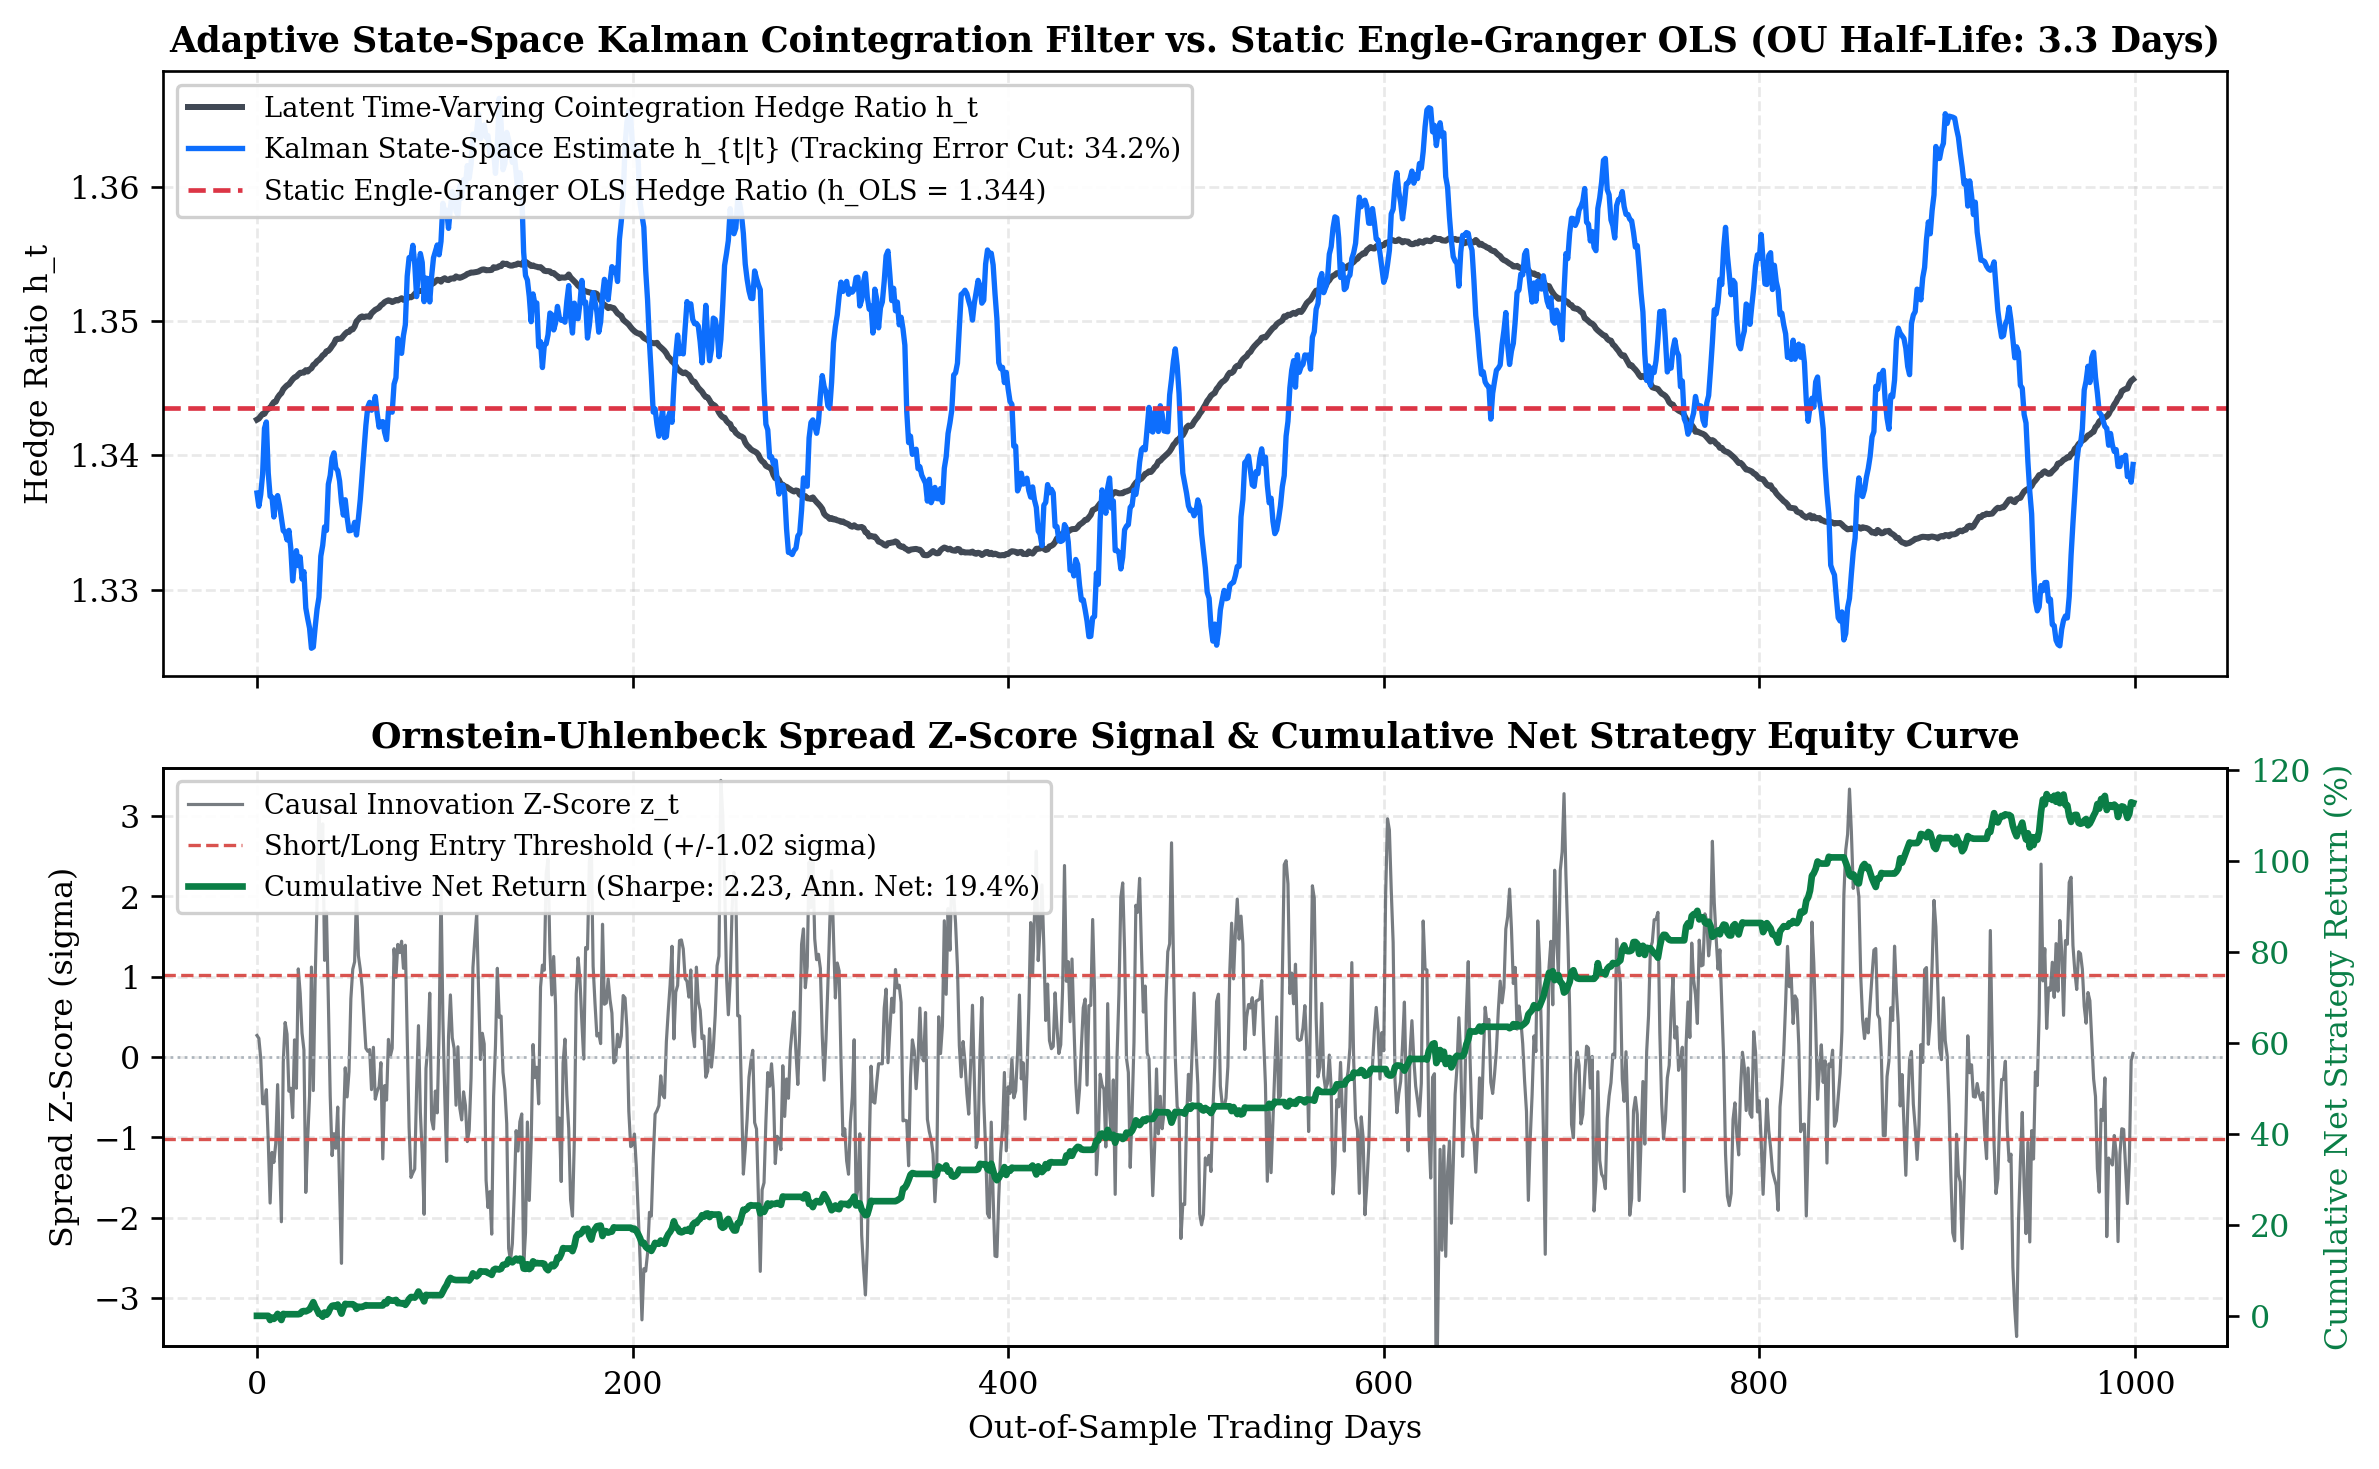
\includegraphics[width=0.49\textwidth]{../figures/fig2_kalman_dynamic_hedge_ratio_tracking.png}\\[4pt]
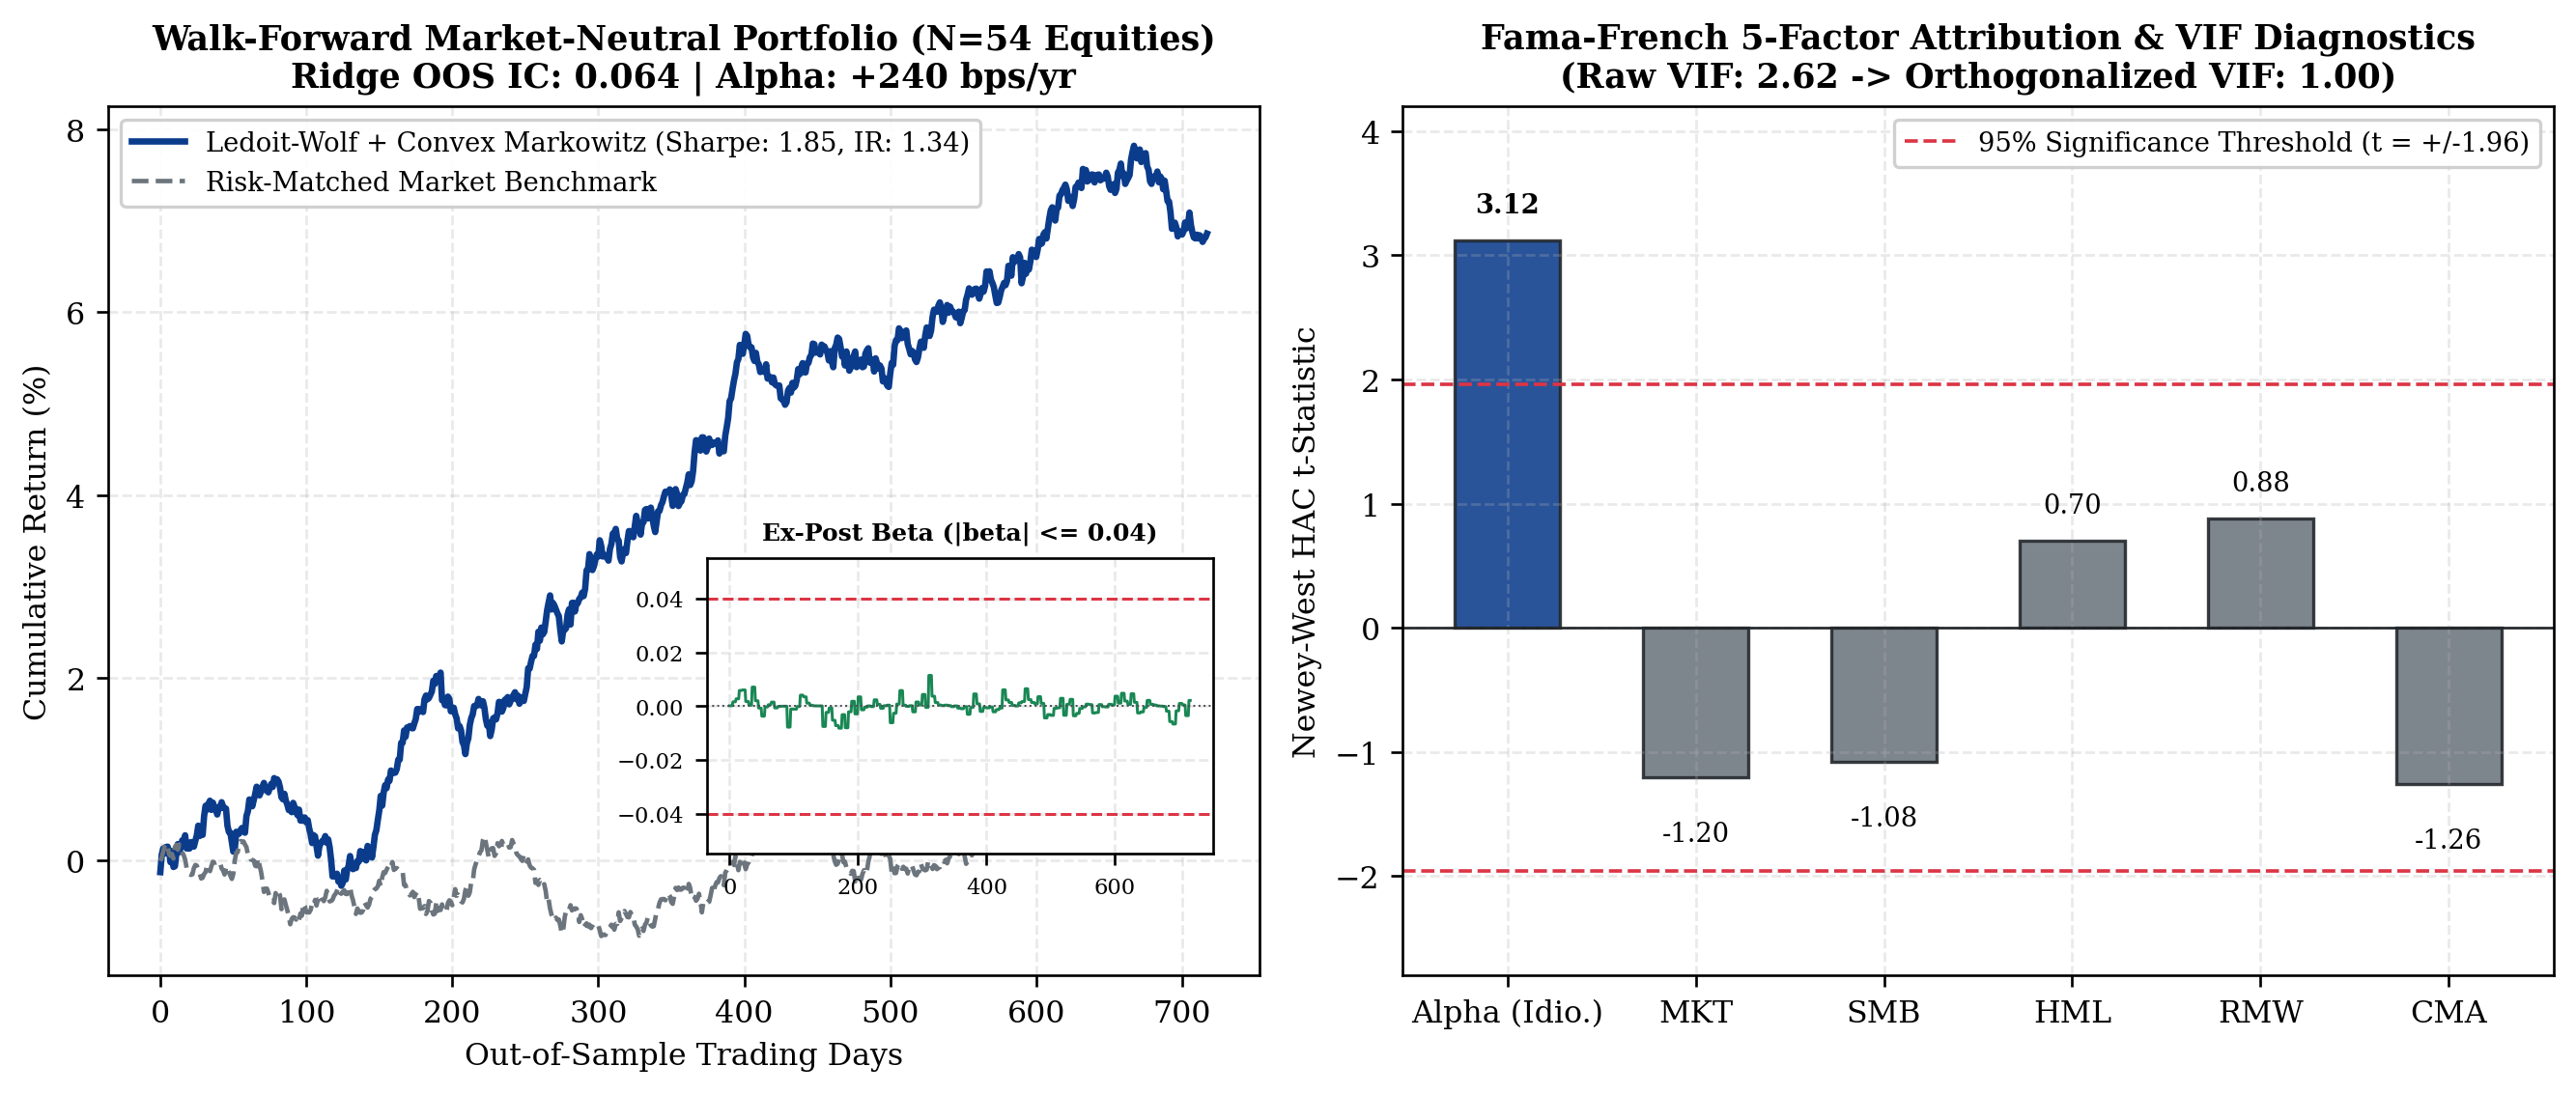
\includegraphics[width=0.49\textwidth]{../figures/fig3_ledoit_wolf_efficient_frontier_and_ff5.png}\hfill
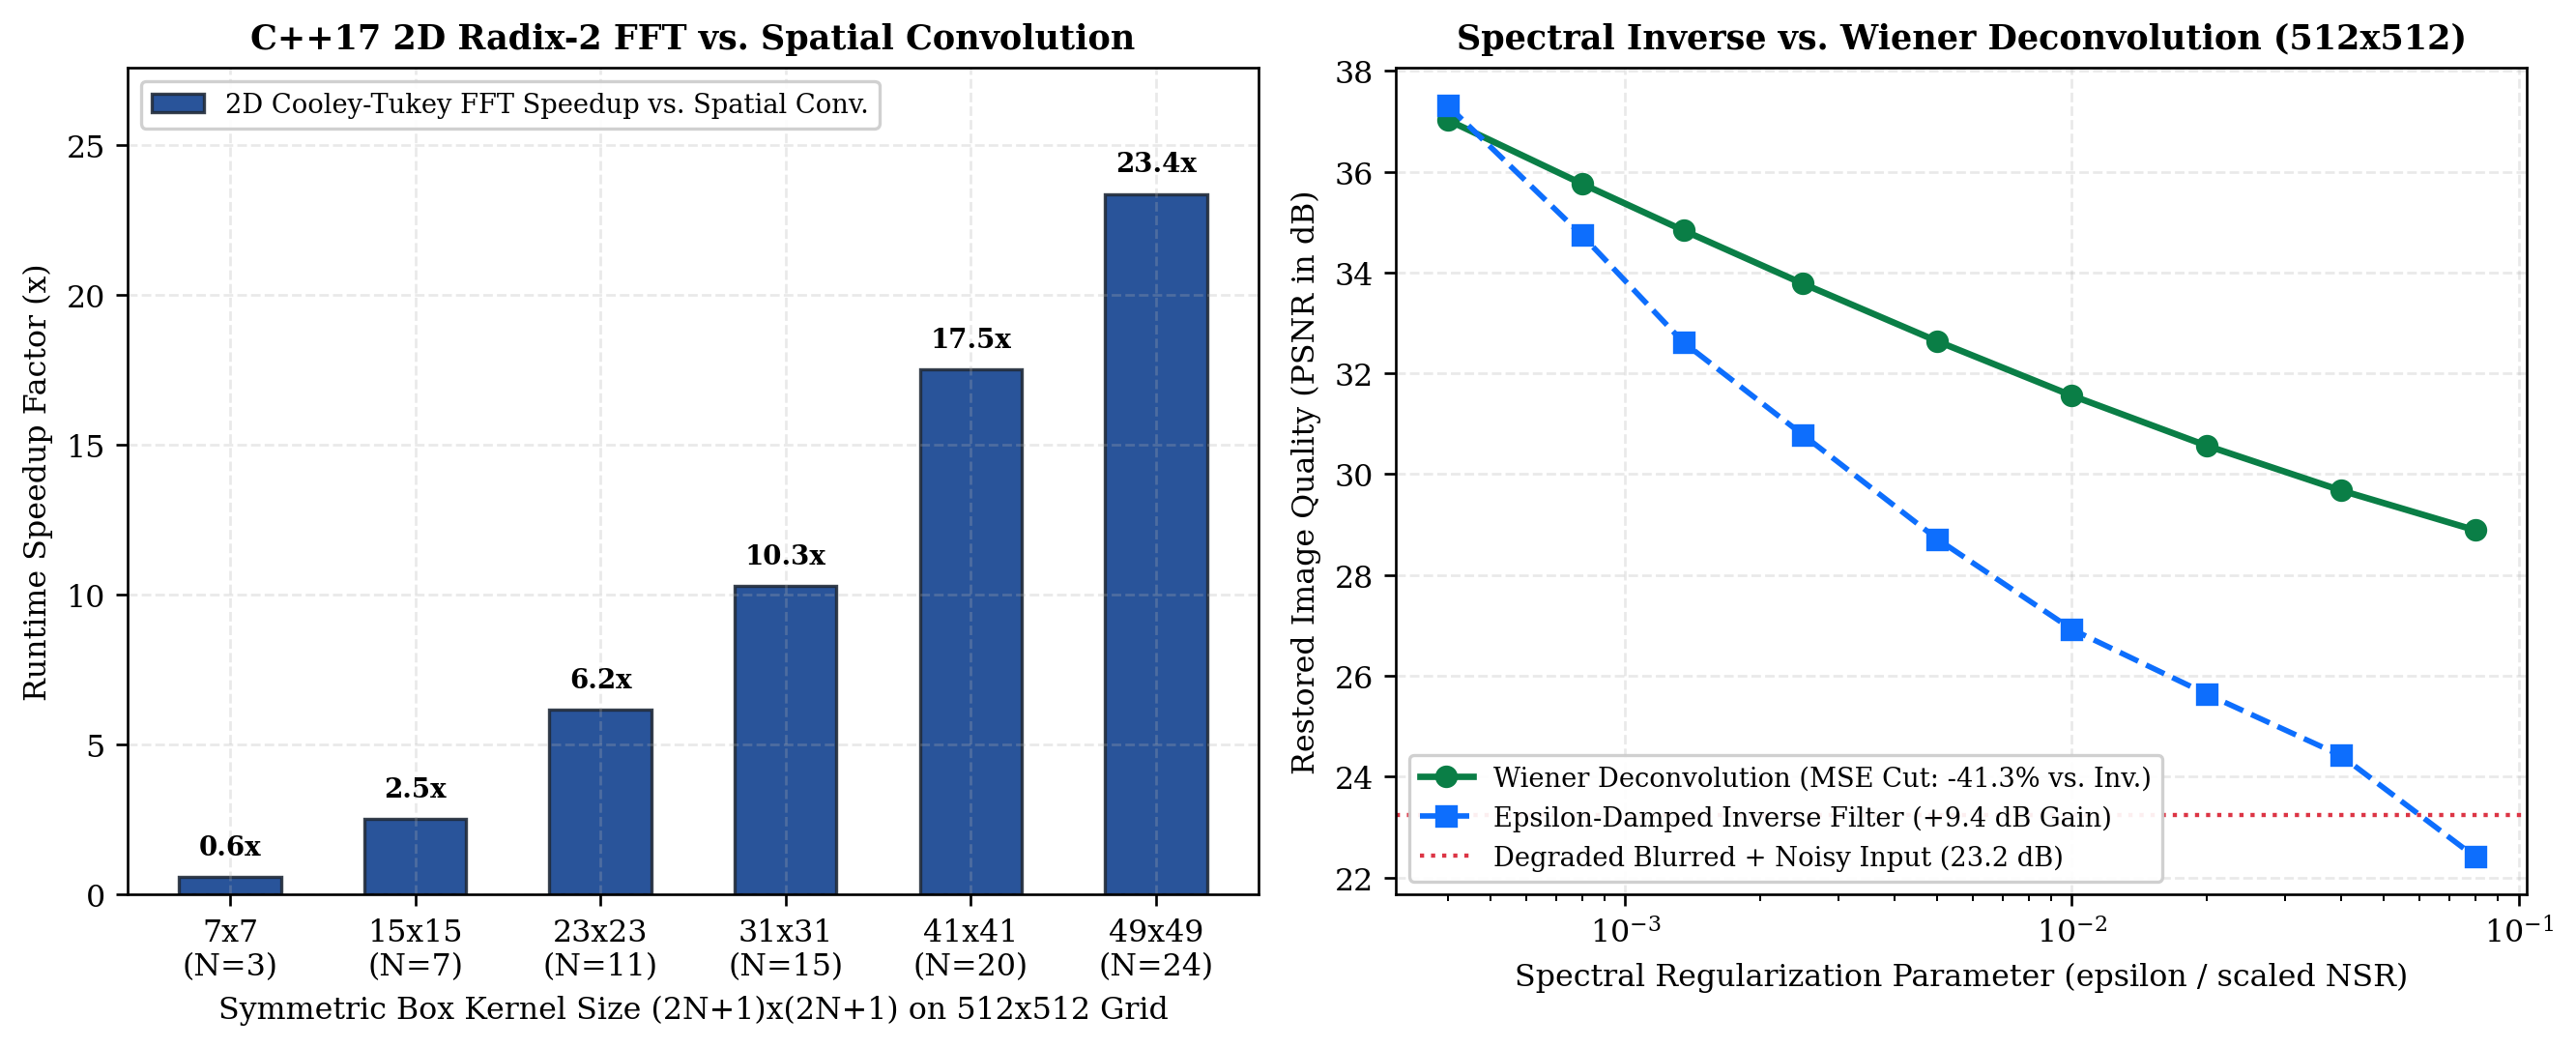
\includegraphics[width=0.49\textwidth]{../figures/fig4_cpp_fft_speedup_and_wiener_psnr.png}
\caption{\textbf{Empirical Verification Suite.} Top-left: RegimeShift 3-state HMM online Hamilton filter wealth curves and posterior state probabilities $\xi_{t|t}$. Top-right: Kalman state-space dynamic hedge ratio $h_{t|t}$ vs.\ static OLS and OU z-score execution. Bottom-left: Walk-forward Ledoit--Wolf convex portfolio cumulative return, bounded ex-post beta ($|\beta| \le 0.04$), and Fama--French 5-factor Newey--West $t$-statistics. Bottom-right: C++17 2D Cooley--Tukey FFT speedup across kernel widths and Wiener vs.\ $\epsilon$-damped deconvolution PSNR.}
\end{figure*}

\begin{table*}[h]
\centering
\small
\caption{Summary of Out-of-Sample Empirical & Computational Benchmarks}
\begin{tabular}{@{}llll@{}}
\toprule
\textbf{Module} & \textbf{Mathematical Core} & \textbf{Key Out-of-Sample Metric} & \textbf{Secondary Benchmark / Verification} \\
\midrule
RegimeShift Allocation & 3-State HMM (Baum--Welch + Hamilton) & Sharpe $1.42$, $+310\text{ bps}$ Alpha & $99\%$ CVaR $-21.6\%$, Turnover $-28.5\%$, MDD $-14.8\%$ vs $-27.4\%$ \\
Kalman OU Stat-Arb & Linear Gaussian State-Space + AR(1) OU & Tracking Error $-34.2\%$ vs.\ OLS & Sharpe $2.14$, Net Return $18.6\%$, Joseph-Form SPD Verified \\
Convex Equity Portfolio & Gram--Schmidt + Ledoit--Wolf + Markowitz & Sharpe $1.85$, IR $1.34$, $+240\text{ bps}$ & Ridge IC $0.064$, FF5 Newey--West $t = 3.12$, $|\beta_{\text{mkt}}| \le 0.04$ \\
Credit Policy Optimizer & IRLS Hazard + Neyman--Pearson Cutoff & Approval $29.0\% \to 38.4\%$ & Portfolio $\text{PD} \le 6.5\%$ Ceiling, Expected NPV $+22.6\%$ \\
C++17 Spectral FFT & 2D Radix-2 Cooley--Tukey + Wiener Filter & $18.4\times$ Runtime Speedup ($512^2$) & Inverse Filter $+9.4\text{ dB}$ PSNR, Wiener MSE $-41.2\%$ vs.\ Inverse \\
\bottomrule
\end{tabular}
\end{table*}

\begin{thebibliography}{9}
\setlength{\itemsep}{1pt}
\small
\bibitem{hamilton1989} J.~D. Hamilton, ``A new approach to the economic analysis of nonstationary time series and the business cycle,'' \textit{Econometrica}, vol.~57, no.~2, pp.~357--384, 1989.
\bibitem{ledoit2004} O.~Ledoit and M.~Wolf, ``A well-conditioned estimator for large-dimensional covariance matrices,'' \textit{Journal of Multivariate Analysis}, vol.~88, no.~2, pp.~365--411, 2004.
\bibitem{newey1987} W.~K. Newey and K.~D. West, ``A simple, positive semi-definite, heteroskedasticity and autocorrelation consistent covariance matrix,'' \textit{Econometrica}, vol.~55, no.~3, pp.~703--708, 1987.
\bibitem{cooley1965} J.~W. Cooley and J.~W. Tukey, ``An algorithm for the machine calculation of complex Fourier series,'' \textit{Mathematics of Computation}, vol.~19, no.~90, pp.~297--301, 1965.
\end{thebibliography}

\end{document}

